Stabil og en av de mest brukte RC-oscillatorene.
Den bruker både positiv og negativ feedback.

\resizebox{\textwidth}{!}{
\begin{circuitikz} \draw
(4.5,4.5) node[op amp] (opamp) {}
(opamp.+) node[left] {}
(opamp.-) node[left] {}
(opamp.out) node[right] {}
(0,4) node[ground] {}
      -- (0,5)
      to[R, l=$R_5$] (2,5)
      to[short, *-] (opamp.-)

%Negativ
(2,5) -- (2,7)
      to[R, l=$R_4$, -*] (7,7)
      to[short, -*] (9,7)
      -- (11,7)
(7,4.5) to[short, -*] (9,4.5)
      to[short, -*] (11,4.5)
      to[short, -o] (12,4.5)
      node[label=$V_{out}$] {}
(7,7) to[R, l=$R_3$] (7,4.5)
(9,4.5) to[D, l=$D_1$, mirror] (9,7)
(11,7) to[D, l=$D_2$] (11,4.5)

%Positiv
(1,0) node[ground] {}
      to[C, l=$C_1$] (1,2)
      to[short, -*] (3,2)
      -- (3,4)
      -- (opamp.+)
(3,0) node[ground] {}
      to[R, l=$R_1$] (3,2)
      to[C, l=$C_2$] (5,2)
      to[R, l=$R_2$] (7,2)
      to[short, -*] (7,4.5)
      -- (opamp.out)
      ;
\end{circuitikz}
} %resizebox




\paragraph{Positiv} \mbox{} \\
Den positive tilbakekoblingen kontrollerer svingningene.

\begin{figure}[H]
  \caption{Resonansfrekvens}
  \centering
  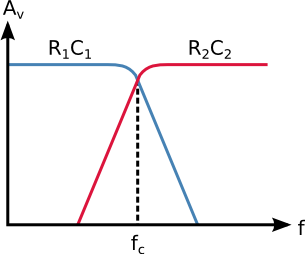
\includegraphics[width=0.5\textwidth]{./img/wien}
\end{figure}

$$R_1 = R_2$$
$$C_1 = C_2$$
$$f_c = \frac{1}{2\pi RC}$$



\paragraph{Negativ} \mbox{} \\
Den negative tilbakekoblingen kontrollerer closed loop gain $A_{CL}$.
Feedback loopen gir en forsterkning, men diodene begrenser spenningen.
$$A_{CL} = \frac{R_f}{R_{inn}} + 1
         = \frac{R_3 + R_4}{R_5} + 1$$

\begin{figure}[H]
  \caption{Diodene clipper signalet ved stor forsterkning}
  \centering
  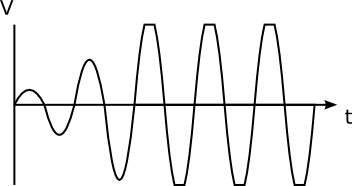
\includegraphics[width=0.5\textwidth]{./img/wienclipp}
\end{figure}
